\chapter{Results} \label{chap:results}

This chapter reports the results in the order of the hypotheses. The main result is the final registered test (seeds 3000--3009); the benchmark and the confirmatory test that preceded it are reported as supporting evidence. Each section gives the results table, the significance tests and a short interpretation tied to one hypothesis. Table~\ref{tab:tests} at the end of the chapter summarises all tests.

\section{Overview of the Experiments}
\label{sec:res-overview}

The evaluation ran in three stages, each on new random seeds (Section~\ref{sec:design}). The \emph{benchmark} (seeds 42--442) compared 12 detectors on 20 drift streams, 9 streams without drift and 9 unannotated real streams (1,584 runs and 396 runs with matched check intervals). It was exploratory: it showed where EADD differs from D3-LightGBM and led to the revised H1. The \emph{confirmatory test} (seeds 1000--1009) tested the revised hypotheses on the 21 drift streams and 8 no-drift streams of Section~\ref{sec:datasets}, with robustness checks for the check schedule (R1) and for constant features (R2). The \emph{final test} (seeds 3000--3009) repeated H1 to H4 once more with every detector on the same check schedule; it has 1,340 stream runs and 10,000 single permutation tests. A comparison with two newer online detectors (seeds 3000--3002) completes the chapter.

Every test was registered before its runs: the hypotheses, data, seeds and decision rule were committed to the public code repository (\texttt{PREREGISTRATION.md}, addenda 0 to 6b) before any result was computed. Analyses formed after seeing the data are marked as exploratory. The unit of analysis is a stream (the mean over its seeds), and the tests are one-sided Wilcoxon signed-rank tests over streams with Holm correction within the registered family (Section~\ref{sec:stats}).

\section{Same-Setup Check and the Parts of EADD}
\label{sec:res-setup}

EADD and D3-LightGBM differ only in the reference window and the permutation test; the classifier, window sizes (500 and 200), threshold ($\tau = 0.7$), 5-fold cross-validation, LightGBM settings, stream objects, seeds and scoring code are identical, and in the final test every detector checks every 50 samples from the same random start (Section~\ref{sec:baselines}). To verify this, EADD's own code was run with its parts switched off (sliding reference, threshold only). On the 20 benchmark drift streams it reproduced D3-LightGBM: recall 0.84 against 0.84 and MTD 299 against 302 samples. Any difference between the two detectors in this chapter therefore comes from EADD's reference and test, not from the setup.

Table~\ref{tab:components} switches EADD's parts on one at a time. The gain comes from the reservoir reference: it raised the gradual recall from 0.00 to 0.50 and the incremental recall from 0.88 to 1.00, and lowered the MTD from 299 to 230 samples. ASPT changed almost no detection at $\tau = 0.7$ (identical results on 19 of 20 streams, and the same mean recall, MTD and false alarms). The classifier matters on slow drift: with the same sliding reference, LightGBM raised the incremental recall from 0.72 (D3, logistic regression) to 0.88. The history null (last row) lowered the false alarms on the drift streams from 4.44 to 3.39 per stream at a small cost in MTD. These differences were not significant on 20 streams (Holm $p \geq 0.51$ for recall), which is why the revised H1 was tested again in two registered tests on new seeds.

\begin{table}[!htbp]
\centering
\caption[Benchmark: the parts of EADD switched on one at a time]{Benchmark (seeds 42--442, 20 drift streams): recall on the gradual and incremental streams, and recall, MTD (samples) and false alarms (FA) per stream over all 20 drift streams, with EADD's parts switched on one at a time. ``Parts off'' is EADD's own code with a sliding reference and no test. Best values in bold.}
\label{tab:components}
\small
\setlength{\tabcolsep}{4pt}
\begin{tabular}{ld{1.2}d{1.2}d{1.2}d{3.0}d{1.2}}
\toprule
 & \multicolumn{2}{c}{Recall} & \multicolumn{3}{c}{All 20 streams} \\
\cmidrule(lr){2-3}\cmidrule(lr){4-6}
Detector & \hd{Gradual} & \hd{Incr.} & \hd{Recall} & \hd{MTD} & \hd{FA} \\
\midrule
D3 (logistic regression) & 0.00 & 0.72 & 0.78 & 415 & \best{1.2}{2.87} \\
D3-LightGBM & 0.00 & 0.88 & 0.84 & 302 & 3.69 \\
\midrule
EADD, parts off & 0.00 & 0.88 & 0.84 & 299 & 3.72 \\
\quad + ASPT & 0.00 & 0.88 & 0.84 & 299 & 3.72 \\
\quad + reservoir & \best{1.2}{0.50} & \best{1.2}{1.00} & \best{1.2}{0.94} & \best{3.0}{230} & 4.44 \\
\quad + reservoir + ASPT & \best{1.2}{0.50} & \best{1.2}{1.00} & \best{1.2}{0.94} & \best{3.0}{230} & 4.44 \\
\quad + reservoir + ASPT + history null (EADD) & \best{1.2}{0.50} & 0.98 & 0.91 & 251 & 3.39 \\
\bottomrule
\end{tabular}
\end{table}

\section{H1: Recall and Detection Delay on Slow Drift}
\label{sec:exp1}

Table~\ref{tab:h1} reports the final test by drift pattern. On gradual drift, EADD detected every drift point (recall 1.00), while D3-LightGBM detected 0.20 and D3 0.28, and EADD's MTD was 582 samples against 1,373 and 1,297. On incremental drift, EADD again reached a recall of 1.00 against 0.85 and 0.68, with an MTD of 304 against 385 and 720 samples. On abrupt drift all three detectors found almost every drift point (D3 missed one drift point in one run), and EADD's MTD of 115 samples was close to D3-LightGBM's 122. When D3-LightGBM did detect an incremental drift it was faster than EADD (a delay of 193 against 304 samples over the detected drift points); its higher MTD on incremental drift (385 against 304) comes from the drift points it missed, which count as the full tolerance. No false alarm was raised on the abrupt streams; on the slow-drift streams EADD raised 1.47 false alarms per stream, D3-LightGBM 2.41 and D3 1.41.

\begin{table}[!htbp]
\centering
\caption[Final test: recall, MTD and delay by drift pattern]{Final test (seeds 3000--3009): recall, mean time to detection (MTD, samples; a miss counts as the tolerance $T$) and mean delay of the detected drift points (samples) on the 7 streams of each drift pattern (one synthetic and six injected), and false alarms (FA) per stream. Slow = the 14 gradual and incremental streams. Best recall, MTD and FA per pattern in bold; none where all three are equal.}
\label{tab:h1}
\small
\setlength{\tabcolsep}{3.5pt}
\begin{tabular}{lld{1.2}d{4.0}d{3.0}d{1.2}}
\toprule
Pattern & Detector & \hd{Recall} & \hd{MTD} & \hd{Delay} & \hd{FA} \\
\midrule
Gradual & EADD & \best{1.2}{1.00} & \best{4.0}{582} & 582 & 0.60 \\
 & D3-LightGBM & 0.20 & 1373 & 852 & \best{1.2}{0.00} \\
 & D3 & 0.28 & 1297 & 780 & \best{1.2}{0.00} \\
\midrule
Incremental & EADD & \best{1.2}{1.00} & \best{4.0}{304} & 304 & \best{1.2}{2.34} \\
 & D3-LightGBM & 0.85 & 385 & 193 & 4.81 \\
 & D3 & 0.68 & 720 & 467 & 2.81 \\
\midrule
Slow (14 streams) & EADD & \best{1.2}{1.00} & \best{4.0}{443} & 443 & 1.47 \\
 & D3-LightGBM & 0.53 & 879 & 522 & 2.41 \\
 & D3 & 0.48 & 1008 & 598 & \best{1.2}{1.41} \\
\midrule
Abrupt & EADD & 1.00 & \best{4.0}{115} & 115 & 0.00 \\
 & D3-LightGBM & 1.00 & 122 & 122 & 0.00 \\
 & D3 & 1.00 & 127 & 125 & 0.00 \\
\bottomrule
\end{tabular}
\end{table}

Table~\ref{tab:h1-tests} gives the registered tests. All three parts of H1 hold after Holm correction against D3-LightGBM, and also against D3: on the 14 slow-drift streams EADD had a higher recall (1.00 against 0.53, Holm $p = 0.015$) and a lower MTD (443 against 879 samples, Holm $p = 0.023$), and on the 7 abrupt streams its MTD was not more than 50 samples higher (115 against 122, Holm $p = 0.023$). The results support H1. Figure~\ref{fig:final-recall-mtd} shows the same comparison.

\begin{table}[!htbp]
\centering
\caption[Final test: registered tests of H1]{Final test: registered one-sided Wilcoxon signed-rank tests of H1 over streams. H1c is a non-inferiority test with a margin of 50 samples. $n$ = number of streams; D3-LGBM = D3-LightGBM. Holm $p$ is corrected within the registered family H1a, H1b, H1c, H2 (Table~\ref{tab:h2-tests}); the tests against D3 are secondary.}
\label{tab:h1-tests}
\small
\setlength{\tabcolsep}{3.5pt}
\begin{tabular}{ld{2.0}rrd{1.3}rd{2.3}}
\toprule
Test & \hd{$n$} & EADD & D3-LGBM & \hd{Holm $p$} & D3 & \hd{Holm $p$} \\
\midrule
H1a: slow-drift recall higher & 14 & 1.00 & 0.53 & 0.015 & 0.48 & 0.005 \\
H1b: slow-drift MTD lower & 14 & 443 & 879 & 0.023 & 1008 & {<}0.001 \\
H1c: abrupt MTD not worse ($+50$) & 7 & 115 & 122 & 0.023 & 127 & 0.016 \\
\bottomrule
\end{tabular}
\end{table}

\begin{figure}[!htbp]
    \centering
    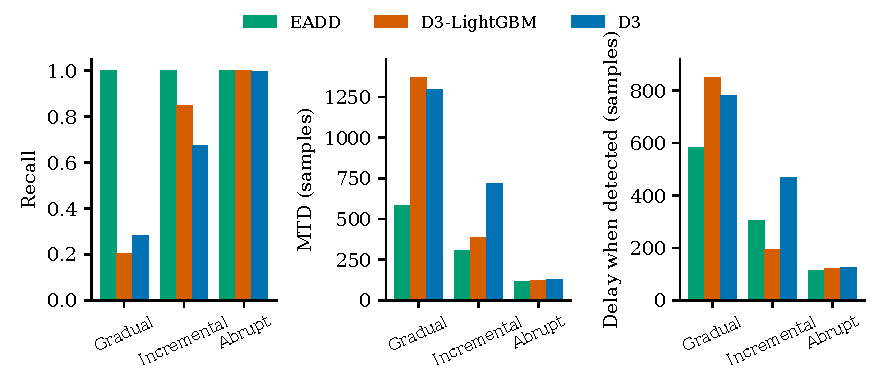
\includegraphics[width=\linewidth]{figures/fig_final_recall_mtd.pdf}
    \caption[Final test: recall, MTD and delay by drift pattern]{Final test (seeds 3000--3009): recall, MTD and delay when detected of EADD, D3-LightGBM and D3 on gradual, incremental and abrupt drift (stream means).}
    \label{fig:final-recall-mtd}
\end{figure}

\paragraph{Replication.} The confirmatory test (seeds 1000--1009, the same 21 drift streams) gave the same result: recall 1.00 against 0.50 (Holm $p = 0.023$), MTD 442 against 890 samples (Holm $p = 0.049$) and abrupt MTD 108 against 119 samples (Holm $p = 0.023$). In that test D3 and D3-LightGBM checked every 51 samples and every seed started at sample 0, so each detector met each drift point at the same phase of its schedule. Robustness check R1 repeated it with every detector checking every 50 samples from a random start, as in the final test, and H1 still held (recall 1.00 against 0.50, Holm $p = 0.017$; MTD 443 against 889, Holm $p = 0.025$; abrupt MTD 115 against 116, Holm $p = 0.017$). Check R2 removed PokerHand and Rialto, on which some shifted features are constant before the drift, which makes those drifts easy to detect: on the 15 remaining streams H1a held (1.00 against 0.45, Holm $p = 0.047$), while H1b (470 against 956) and H1c (112 against 124) had raw $p$ of 0.042 and 0.031 and Holm $p$ of 0.063, just above 0.05, with 10 and 5 streams respectively.

\section{H2: False Alarms}
\label{sec:exp2}

H2 is measured on streams without drift, where every alarm is false. Table~\ref{tab:h2} gives the false alarms per 10,000 samples. On the six autocorrelated AR(1) streams ($\rho$ from 0.8 to 0.97), EADD raised 5.59 false alarms per 10,000 samples, D3-LightGBM 19.5 and D3 18.5. EADD raised fewer than D3-LightGBM on all six streams, about 3.5 times fewer (one-sided Wilcoxon, Holm $p = 0.023$ against D3-LightGBM, the primary comparison; Holm $p = 0.016$ against D3, the secondary comparison). The results support H2. D3-LightGBM's 19.5 is close to the most it can raise: after an alarm it needs a new 500-sample reference before the next check, so it alarmed at almost every opportunity on these streams. The result therefore shows that the history-null test removes most of these alarms, not that the two detectors were close. On the 8 other no-drift streams (synthetic, shuffled real, AR 0.5 and AR 0.9), EADD raised 0.75 false alarms per 10,000 samples against 2.44 and 2.41; all of EADD's and almost all of the baselines' false alarms there came from the AR 0.9 stream, and none of the three detectors raised a false alarm on the synthetic and shuffled real streams. Figure~\ref{fig:final-fa} shows both groups.

\paragraph{Source of the effect (addendum 7b).} Two further EADD variants were run on the six autocorrelated streams (seeds 3000--3004), each with one component changed. With the reservoir reference but the usual label-shuffle null, EADD raised 19.5 false alarms per 10,000 samples on every stream, the same as D3-LightGBM. With a sliding reference, as in D3, but the history null, it raised 4.15, close to EADD's 5.65 on the same seeds; it was lower than the label-shuffle variant on all six streams (one-sided Wilcoxon, $p = 0.016$, the smallest value possible with six streams). The reduction in false alarms therefore comes from the history null, not from the reservoir reference.

\begin{table}[!htbp]
\centering
\caption[Final test: false alarms on streams without drift]{Final test: false alarms per 10,000 samples on the streams without drift (mean over 10 seeds). The registered H2 test is on the six autocorrelated streams. Fewest false alarms per row in bold.}
\label{tab:h2}
\small
\begin{tabular}{ld{1.2}d{2.2}d{2.2}}
\toprule
Stream & \hd{EADD} & \hd{D3-LightGBM} & \hd{D3} \\
\midrule
AR 0.80 & \best{1.2}{5.00} & 19.50 & 15.35 \\
AR 0.85 & \best{1.2}{4.50} & 19.50 & 18.15 \\
AR 0.90 & \best{1.2}{6.00} & 19.50 & 19.25 \\
AR 0.93 & \best{1.2}{5.60} & 19.50 & 19.45 \\
AR 0.95 & \best{1.2}{6.30} & 19.50 & 19.50 \\
AR 0.97 & \best{1.2}{6.15} & 19.50 & 19.50 \\
\midrule
Mean, autocorrelated (6) & \best{1.2}{5.59} & 19.50 & 18.53 \\
Mean, other no-drift streams (8) & \best{1.2}{0.75} & 2.44 & 2.41 \\
\bottomrule
\end{tabular}
\end{table}

\begin{table}[!htbp]
\centering
\caption[Final test: registered test of H2]{Final test: registered one-sided Wilcoxon signed-rank test of H2 over the six autocorrelated streams without drift (false alarms per 10,000 samples). Holm $p$ is corrected within the family of Table~\ref{tab:h1-tests}.}
\label{tab:h2-tests}
\small
\begin{tabular}{ld{1.0}d{1.2}d{2.2}d{1.3}d{2.2}d{1.3}}
\toprule
Test & \hd{Streams} & \hd{EADD} & \hd{D3-LightGBM} & \hd{Holm $p$} & \hd{D3} & \hd{Holm $p$} \\
\midrule
H2: fewer false alarms & 6 & 5.59 & 19.50 & 0.023 & 18.53 & 0.016 \\
\bottomrule
\end{tabular}
\end{table}

\begin{figure}[!htbp]
    \centering
    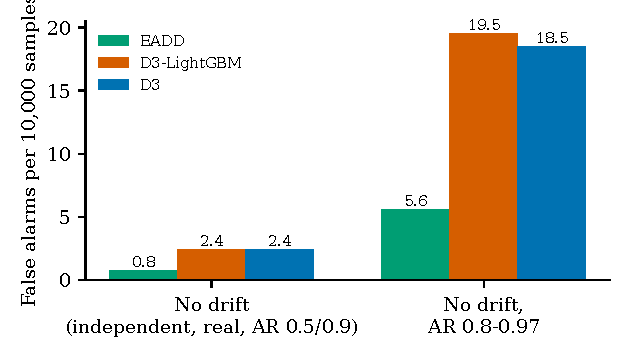
\includegraphics[width=\linewidth]{figures/fig_final_false_alarms.pdf}
    \caption[Final test: false alarms without drift]{Final test: false alarms per 10,000 samples of EADD, D3-LightGBM and D3 on the no-drift streams (synthetic, shuffled real, AR 0.5 and 0.9) and on the autocorrelated no-drift streams (AR 0.8 to 0.97).}
    \label{fig:final-fa}
\end{figure}

\paragraph{How H2 reached this form.} In the confirmatory test, H2 was registered on the 8 no-drift streams together with a validity condition at AR 0.9. It was not supported: EADD raised 0.62 false alarms per 10,000 samples against 2.44 ($p = 0.50$), because only one stream had any false alarm, and the test rejected 7.0\% (steady state) and 9.4\% (after an alarm) of the no-drift tests at AR 0.9. The test on autocorrelated streams was then registered (addendum 3) and run on new seeds 2000--2009: EADD raised 4.46 against 19.5 false alarms per 10,000 samples, fewer on 6 of 6 streams ($p = 0.016$). The final test repeated it on seeds 3000--3009 with the result above.

\paragraph{Validity of the test.} The share of no-drift tests that EADD's permutation test rejects was measured as a descriptive result, with 1,000 tests in each of ten conditions (Table~\ref{tab:validity}, Figure~\ref{fig:test-validity}). At $\alpha = 0.05$ the rejection rates were between 3.8\% and 6.9\%; seven of the ten conditions had a one-sided 95\% Clopper--Pearson upper bound of at most 0.075, and the three others were AR 0.3 and AR 0.5 in the steady state (6.5\% and 6.6\%) and shuffled Electricity at the first test after an alarm (6.9\%). At EADD's own alarm rule ($p \leq 2\alpha/3 \approx 0.033$), the steady-state rates were between 2.9\% and 4.2\%.

\begin{table}[!htbp]
\centering
\caption[Final test: rejection rates of the test without drift]{Final test (descriptive): share of 1,000 no-drift tests per condition with $p \leq 0.05$, its one-sided 95\% Clopper--Pearson upper bound, and the share with $p \leq 0.033$ (EADD's alarm rule). Steady = a long history of earlier windows; After alarm = the first test after an alarm; then only 31 null draws exist, so $p$ takes steps of 1/32 and the two thresholds reject the same tests.}
\label{tab:validity}
\small
\begin{tabular}{lld{1.3}d{1.3}d{1.3}}
\toprule
Data & State & \hd{$p \leq 0.05$} & \hd{Upper bound} & \hd{$p \leq 0.033$} \\
\midrule
Gaussian, independent & Steady & 0.051 & 0.064 & 0.036 \\
 & After alarm & 0.057 & 0.071 & 0.057 \\
\addlinespace
Shuffled Electricity & Steady & 0.055 & 0.068 & 0.035 \\
 & After alarm & 0.069 & 0.084 & 0.069 \\
\addlinespace
Shuffled PokerHand & Steady & 0.055 & 0.068 & 0.029 \\
 & After alarm & 0.048 & 0.061 & 0.048 \\
\addlinespace
AR 0.3 & Steady & 0.065 & 0.079 & 0.035 \\
 & After alarm & 0.038 & 0.050 & 0.038 \\
\addlinespace
AR 0.5 & Steady & 0.066 & 0.080 & 0.042 \\
 & After alarm & 0.056 & 0.070 & 0.056 \\
\bottomrule
\end{tabular}
\end{table}

\begin{figure}[!htbp]
    \centering
    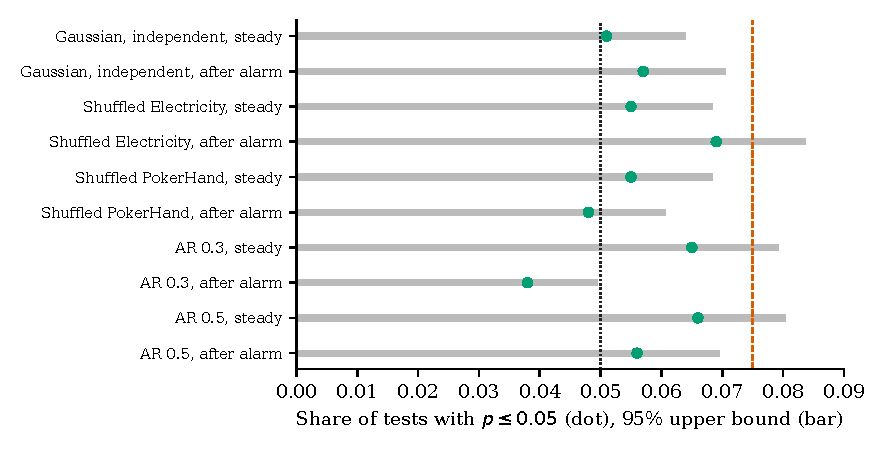
\includegraphics[width=\linewidth]{figures/fig_test_validity.pdf}
    \caption[Rejection rates of the test without drift]{Share of no-drift tests with $p \leq 0.05$ (dot) and its one-sided 95\% Clopper--Pearson upper bound (bar) in the ten conditions of Table~\ref{tab:validity}. Dotted line: the nominal 0.05; dashed line: 0.075.}
    \label{fig:test-validity}
\end{figure}

\section{H3: ASPT against the Full Permutation Test}
\label{sec:exp3}

H3 was tested as equivalence (TOST, two one-sided Wilcoxon tests) between EADD with ASPT and EADD with the full permutation test (199 draws, same null and alarm rule), within margins of 0.05 recall, 50 samples MTD and 0.5 false alarms per stream on the 21 drift streams, and 1.0 false alarms per 10,000 samples on the 8 no-drift streams. Table~\ref{tab:h3} shows that all four measures were equivalent. ASPT used 52 permutations per test against 163 for the full test, over the 22 streams on which tests ran ($p < 0.001$; the full test averages fewer than 199 because the history null caps the draws at the number of earlier windows, Section~\ref{sec:eadd-algorithm}); on the abrupt streams every ASPT test stopped after 59 permutations. The results support H3. Figure~\ref{fig:aspt} compares the two tests stream by stream.

\begin{table}[!htbp]
\centering
\caption[Final test: ASPT against the full permutation test]{Final test: EADD with ASPT and with the full permutation test. H3a: TOST equivalence (both one-sided Wilcoxon tests over streams significant; the larger $p$ is shown). H3b: one-sided Wilcoxon test of the permutations per test.}
\label{tab:h3}
\small
\setlength{\tabcolsep}{3.5pt}
\begin{tabular}{ld{2.0}d{2.2}d{3.2}d{3.2}d{2.3}}
\toprule
Test & \hd{Streams} & \hd{Margin} & \hd{ASPT} & \hd{Full test} & \hd{$p$} \\
\midrule
H3a: recall equivalent & 21 & 0.05 & 1.00 & 1.00 & {<}0.001 \\
H3a: MTD equivalent & 21 & 50 & 333.7 & 333.5 & {<}0.001 \\
H3a: FA per stream equivalent & 21 & 0.5 & 0.98 & 0.96 & {<}0.001 \\
H3a: FA per 10k (no drift) equivalent & 8 & 1.0 & 0.75 & 0.63 & 0.008 \\
H3b: fewer permutations per test & 22 & & 51.9 & 162.6 & {<}0.001 \\
\bottomrule
\end{tabular}
\end{table}

\begin{figure}[!htbp]
    \centering
    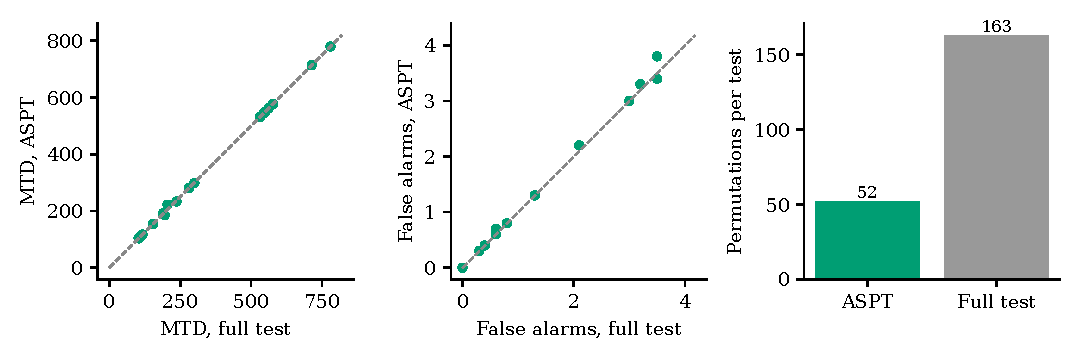
\includegraphics[width=\linewidth]{figures/fig_aspt_equivalence.pdf}
    \caption[Final test: ASPT against the full test]{Final test: MTD and false alarms per drift stream of EADD with ASPT against the full permutation test (dotted line: equal values), and the mean number of permutations per test.}
    \label{fig:aspt}
\end{figure}

Wall-clock time was measured separately, with one run at a time on the four annotated INSECTS streams (5 seeds, 20 run pairs), with the corrected options but the label-shuffle null instead of the history null, which explains the 199 draws of every full test. EADD with ASPT spent 210 seconds per run in the detector against 453 seconds with the full test, 54\% less, and was faster in 20 of 20 runs (one-sided paired Wilcoxon $p < 0.001$); the two gave identical detections in 20 of 20 runs. Over these runs ASPT used 18,408 permutations for 312 tests (59 per test) against 62,088 (199 per test). EADD without any test took 116 seconds per run, so most of the remaining time is spent training the classifier at every check.

\paragraph{Wall-clock time with the history null (addendum 7c).} The same comparison was repeated with the history null of the final test on the four INSECTS streams with seeds 42 and 142 (8 run pairs, in alternating order). EADD with ASPT spent 322 seconds per run in the detector against 569 seconds with the full test, 43\% less, and was faster in 8 of 8 runs (one-sided paired Wilcoxon $p = 0.004$). ASPT used 83 permutations per test against 168; the full test averages fewer than 199 because after an alarm the history holds fewer earlier windows. The detections were identical in 3 of the 8 runs: when the two tests decide one check differently, the reference after it differs as well, so the later detections of the run can differ. Detection quality is compared by the registered H3a test above. The runs were made on a laptop that was also used for short document builds during the measurement; the alternating order spreads this load over both tests.

In the confirmatory test, H3a had been registered under a stricter rule: identical detections in at least 95\% of the 290 run pairs. The two tests gave identical detections in 81\% of the pairs and the same recall, MTD and false alarms, so H3a was not supported under that rule; the final test registered the equivalence formulation above, which measures the detection quality directly.

\section{H4: Feature Attribution at a Detection}
\label{sec:exp4}

H4 concerns TreeSHAP attribution \citep{LundbergInteraction2020} in a classifier-based drift detector: at the first detection of each drift point, the features ranked highest should be the features that truly drift. It was measured with EADD's runs on the 21 drift streams of the final test, where the drifting features are known. Precision@$k$ ($k$ = the number of drifting features) was 0.75, against a chance level $k/d$ of 0.31 (one-sided Wilcoxon over streams, $p < 0.001$), and the top-ranked feature was a drifting feature in 98.4\% of the detections. The results support H4. Precision was close to 1.00 on the three synthetic streams and lowest on Rialto (0.45 to 0.48, chance 0.30). Without PokerHand and Rialto, whose shifted features include features that are constant before the drift (which makes those drifts easy to detect), precision@$k$ was 0.80 against 0.32 (15 streams). The confirmatory test gave the same result (0.75 against 0.31, top-1 99\%; 0.81 against 0.32 without PokerHand and Rialto). Figure~\ref{fig:h4} shows every stream.

\paragraph{Comparison with univariate rankings (addendum 7a).} At the same detections (the rerun reproduced all 210 runs exactly), the features were also ranked by two univariate statistics computed from the same two windows: the two-sample Kolmogorov--Smirnov (KS) statistic and the absolute standardised mean difference (SMD). The KS ranking reached a precision@$k$ of 0.97 and the SMD ranking 0.89, against 0.75 for TreeSHAP; TreeSHAP was higher on only 1 and 4 of the 21 streams (two-sided Wilcoxon, Holm $p < 0.001$ and $p = 0.010$). In these streams every drift moves the marginal distribution of single features, which a per-feature statistic measures directly. A drift that changes only the dependence between features, where the classifier's attribution could have an advantage, was not part of the test.

\begin{figure}[!htbp]
    \centering
    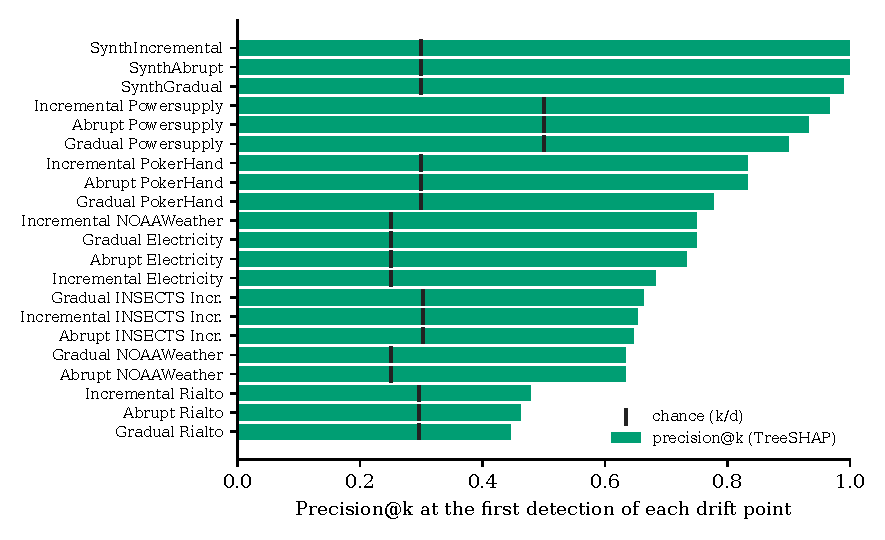
\includegraphics[width=\linewidth]{figures/fig_h4_precision.pdf}
    \caption[Final test: precision@$k$ of TreeSHAP attribution]{Final test: precision@$k$ of the TreeSHAP ranking at the first detection of each drift point (bars) and the chance level $k/d$ (marks) on the 21 drift streams, measured with EADD.}
    \label{fig:h4}
\end{figure}

\section{Comparison with Newer Online Detectors}
\label{sec:newer}

EADD was also compared with MMD-Online, LSDD-Online \citep{CobbSequential2022} and CVM-Online \citep{RossAdams2012} from Alibi Detect \citep{AlibiDetect}, three unsupervised online detectors calibrated to an expected run time of 2,500 samples without drift (window 50, 25,000 bootstrap draws for MMD-Online and LSDD-Online and 100,000 for CVM-Online, a new 500-sample reference after each alarm). Their recalibration after every alarm is slow, so this comparison was registered on seeds 3000--3002 only, and EADD, D3-LightGBM and D3 are shown as their means over the same three seeds. CVM-Online was rerun with 100,000 draws as registered in addendum 6b, because with 25,000 its per-feature thresholds could not be estimated on streams with many features.

Table~\ref{tab:newer} shows a trade-off between delay and false alarms. The online detectors detected slow drift sooner than EADD: CVM-Online had a recall of 1.00 and the lowest MTD on slow drift (224 samples), and LSDD-Online had a recall of 1.00, an MTD of 365 samples on slow drift and the lowest MTD on abrupt drift (66). They raised many more false alarms: 9.88 (CVM-Online) and 7.67 (LSDD-Online) per slow-drift stream and 7.67 and 6.24 per abrupt stream, against 1.52 and 0 for EADD. MMD-Online had a recall of 0.94 on slow and 0.84 on abrupt drift with a similar number of false alarms. On the streams without drift the online detectors raised 6.82 to 7.13 false alarms per 10,000 samples against 0.75 for EADD, and on the autocorrelated streams 18.0 to 19.2 against 5.89. Figure~\ref{fig:newer} plots MTD against false alarms.

\begin{table}[!htbp]
\centering
\caption[Comparison with newer online detectors]{Newer online detectors (seeds 3000--3002): recall, MTD (samples) and false alarms (FA) per stream on the 14 slow-drift and 7 abrupt streams, and false alarms per 10,000 samples on the 8 no-drift and 6 autocorrelated streams. Best values in bold.}
\label{tab:newer}
\small
\setlength{\tabcolsep}{3pt}
\begin{tabular}{ld{1.2}d{4.0}d{1.2}d{1.2}d{3.0}d{1.2}d{1.2}d{2.2}}
\toprule
 & \multicolumn{3}{c}{Slow drift} & \multicolumn{3}{c}{Abrupt drift} & \multicolumn{2}{c}{FA per 10k} \\
\cmidrule(lr){2-4}\cmidrule(lr){5-7}\cmidrule(lr){8-9}
Detector & \hd{Recall} & \hd{MTD} & \hd{FA} & \hd{Recall} & \hd{MTD} & \hd{FA} & \hd{No drift} & \hd{AR} \\
\midrule
EADD & \best{1.2}{1.00} & 443 & 1.52 & \best{1.2}{1.00} & 114 & \best{1.2}{0.00} & \best{1.2}{0.75} & \best{2.2}{5.89} \\
CVM-Online & \best{1.2}{1.00} & \best{4.0}{224} & 9.88 & 0.97 & 78 & 7.67 & 7.13 & 18.00 \\
LSDD-Online & \best{1.2}{1.00} & 365 & 7.67 & 0.97 & \best{3.0}{66} & 6.24 & 6.82 & 19.06 \\
MMD-Online & 0.94 & 463 & 6.88 & 0.84 & 133 & 5.57 & 6.84 & 19.22 \\
D3-LightGBM & 0.52 & 894 & 2.38 & \best{1.2}{1.00} & 124 & \best{1.2}{0.00} & 2.44 & 19.50 \\
D3 & 0.43 & 1058 & \best{1.2}{1.26} & \best{1.2}{1.00} & 129 & \best{1.2}{0.00} & 2.40 & 18.61 \\
\bottomrule
\end{tabular}
\end{table}

\begin{figure}[!htb]
    \centering
    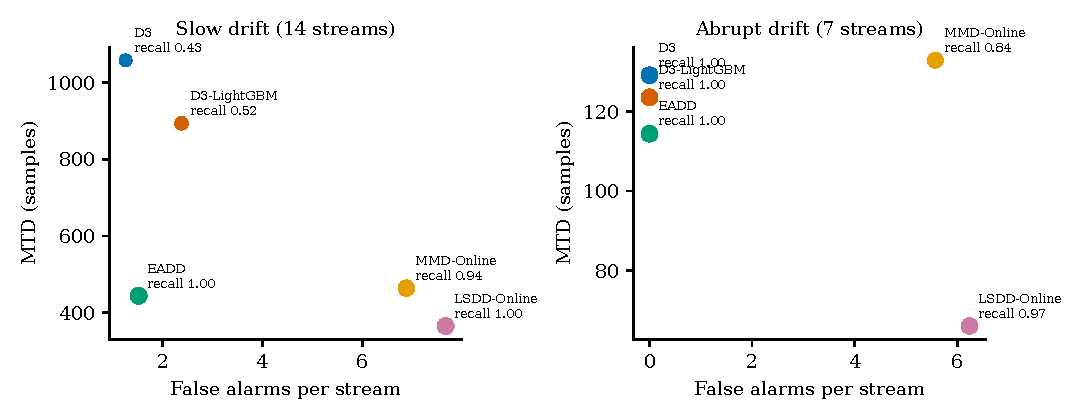
\includegraphics[width=\linewidth]{figures/fig_newer_detectors.pdf}
    \caption[Newer online detectors: MTD against false alarms]{Newer online detectors (seeds 3000--3002): MTD against false alarms per stream on slow and abrupt drift; Table~\ref{tab:newer} gives the recall.}
    \label{fig:newer}
\end{figure}

Table~\ref{tab:friedman} gives the Friedman mean ranks over the 21 drift streams (1 = best; Friedman $p \leq 0.001$ for each metric; Nemenyi critical difference 1.65). EADD had the best mean rank for recall, although no recall difference exceeded the critical difference. CVM-Online had the best rank for MTD and was better than EADD, D3-LightGBM and D3 by more than the critical difference; LSDD-Online and MMD-Online were better than D3, and LSDD-Online also than D3-LightGBM. For false alarms, EADD's rank (2.19) was better than that of each online detector (4.57 to 5.14) by more than the critical difference. The registered pairwise tests of EADD against each online detector (the H1 and H2 tests, Holm over 12 tests) were not significant: with 3 seeds the tests were underpowered, and the smallest Holm $p$ was 0.19 (H2, raw $p = 0.016$ against each online detector).

\begin{table}[!htbp]
\centering
\caption[Friedman mean ranks with the newer detectors]{Friedman mean ranks over the 21 drift streams (seeds 3000--3002; 1 = best). Nemenyi critical difference 1.65. Best ranks in bold.}
\label{tab:friedman}
\small
\begin{tabular}{ld{1.2}d{1.2}d{1.2}}
\toprule
Detector & \hd{Recall} & \hd{MTD} & \hd{False alarms} \\
\midrule
EADD & \best{1.2}{2.83} & 3.67 & 2.19 \\
CVM-Online & 3.10 & \best{1.2}{1.90} & 5.14 \\
LSDD-Online & 3.10 & 2.76 & 5.02 \\
MMD-Online & 3.52 & 3.24 & 4.57 \\
D3-LightGBM & 4.17 & 4.43 & 2.26 \\
D3 & 4.29 & 5.00 & \best{1.2}{1.81} \\
\bottomrule
\end{tabular}
\end{table}

\section{Annotated Real Streams (INSECTS)}
\label{sec:insects}

The four INSECTS streams \citep{Souza2020} are the only real streams with documented drift points. They were used in the benchmark (seeds 42--442) and not in the registered tests, so these results are exploratory. Table~\ref{tab:insects} compares EADD (with the history null) with D3-LightGBM and D3, all checking every 50 samples. EADD was not better on these streams. On abrupt drift the three detectors were close; on gradual drift none detected a drift point within the tolerance of 500 samples; on the two incremental streams EADD found fewer drift points (0.80 and 0.60 against 1.00) and raised more alarms counted as false.

\begin{table}[!htbp]
\centering
\caption[Benchmark: annotated INSECTS streams]{Benchmark (seeds 42--442): recall, MTD (samples) and alarms counted as false (FA) per stream on the four annotated INSECTS streams, all detectors checking every 50 samples. Rec. = recall; EADD = EADD with the history null (stride 10). Best value of each measure per stream in bold; none where all three are equal.}
\label{tab:insects}
\small
\begin{tabular}{ld{1.2}d{3.0}d{2.1}d{1.2}d{3.0}d{2.1}d{1.2}d{3.0}d{2.1}}
\toprule
 & \multicolumn{3}{c}{EADD} & \multicolumn{3}{c}{D3-LightGBM} & \multicolumn{3}{c}{D3} \\
\cmidrule(lr){2-4}\cmidrule(lr){5-7}\cmidrule(lr){8-10}
Stream & \hd{Rec.} & \hd{MTD} & \hd{FA} & \hd{Rec.} & \hd{MTD} & \hd{FA} & \hd{Rec.} & \hd{MTD} & \hd{FA} \\
\midrule
Abrupt & \best{1.2}{0.84} & 180 & 6.0 & 0.80 & \best{3.0}{172} & 6.0 & 0.80 & 180 & 6.0 \\
Gradual & 0.00 & 500 & 6.0 & 0.00 & 500 & 5.4 & 0.00 & 500 & \best{2.1}{5.0} \\
Incremental-abrupt & 0.80 & 212 & 18.8 & \best{1.2}{1.00} & \best{3.0}{95} & 13.4 & \best{1.2}{1.00} & 99 & \best{2.1}{10.4} \\
Incremental-reoccurring & 0.60 & 309 & 20.2 & \best{1.2}{1.00} & \best{3.0}{246} & 14.2 & \best{1.2}{1.00} & 272 & \best{2.1}{13.4} \\
\bottomrule
\end{tabular}
\end{table}

\section{Unannotated Real Streams}
\label{sec:unannotated}

On the nine unannotated real streams of the benchmark, following \citet{Lukats2024}, a Hoeffding tree was retrained at every detection and its prequential accuracy was measured (Table~\ref{tab:e4-acc}). The accuracies of all detectors were within a few percentage points of each other: EADD 65.0\%, D3-LightGBM 66.7\% and D3 66.8\%, with IBDD highest at 68.3\%. EADD raised far fewer detections (216 in total over the nine streams, against 524 for D3-LightGBM and 499 for D3). Accuracy rewards frequent retraining \citep{Lukats2024}, so this table does not show which detector finds the real changes; it is reported for completeness and does not test a hypothesis.

\begin{table}[!htbp]
\centering
\caption[Benchmark: classifier accuracy on the unannotated streams]{Benchmark (seeds 42, 142, 242): prequential accuracy (\%) of a Hoeffding tree retrained at every detection on the nine unannotated streams, their mean, and the total number of detections (Det.) over the nine streams (mean over seeds). Columns: Electricity, INSECTS Incremental, Luxembourg, NOAAWeather, OutdoorObjects, Ozone, PokerHand, Powersupply, RialtoBridgeTimelapse.}
\label{tab:e4-acc}
\footnotesize
\setlength{\tabcolsep}{2.5pt}
\begin{tabular}{l*{10}{d{2.1}}d{4.0}}
\toprule
Detector & \hd{Elec.} & \hd{Incr.} & \hd{Lux.} & \hd{NOAA} & \hd{Outdoor} & \hd{Ozone} & \hd{Poker} & \hd{Power} & \hd{Rialto} & \hd{Mean} & \hd{Det.} \\
\midrule
EADD & 80.2 & 52.0 & 97.2 & 69.8 & 59.8 & 93.7 & 67.0 & 14.3 & 51.3 & 65.0 & 216 \\
D3-LightGBM & 82.3 & 50.3 & 90.0 & 70.4 & 71.0 & 93.6 & 70.7 & 16.4 & 55.4 & 66.7 & 524 \\
D3 & 82.3 & 50.3 & 95.8 & 70.0 & 68.7 & 93.6 & 69.8 & 16.4 & 54.3 & 66.8 & 499 \\
BNDM & 81.7 & 55.1 & 95.7 & 70.3 & 65.3 & 93.7 & 67.3 & 16.2 & 48.0 & 65.9 & 268 \\
CSDDM & 82.1 & 56.3 & 95.6 & 71.5 & 66.1 & 93.7 & 69.8 & 16.8 & 54.8 & 67.4 & 572 \\
IBDD & 82.9 & 51.9 & 90.0 & 69.1 & 78.0 & 93.6 & 77.0 & 21.1 & 51.5 & 68.3 & 9411 \\
OCDD & 82.5 & 53.7 & 93.2 & 70.7 & 65.5 & 93.7 & 69.3 & 16.7 & 53.9 & 66.6 & 657 \\
SPLL & 82.0 & 50.9 & 95.7 & 71.4 & 66.1 & 93.7 & 68.3 & 15.4 & 54.6 & 66.5 & 396 \\
UDetect & 79.9 & 50.9 & 97.6 & 73.5 & 59.6 & 93.7 & 65.2 & 16.2 & 31.1 & 63.1 & 0 \\
\bottomrule
\end{tabular}
\end{table}

\section{Summary of the Hypothesis Tests}

The four hypotheses, as stated in Section~\ref{sec:intro-hypotheses}, were:
\begin{description}
    \item[H1:] \hypHone
    \item[H2:] \hypHtwo
    \item[H3:] \hypHthree
    \item[H4:] \hypHfour
\end{description}
Table~\ref{tab:tests} summarises their registered tests in the final test. All four hypotheses are supported: H1a, H1b and H1c against D3-LightGBM, H2 against D3-LightGBM (primary) and D3 (secondary), H3a and H3b, and H4, measured with EADD.

\begin{table}[!htbp]
\centering
\caption[Summary of the hypothesis tests]{Summary of the registered hypothesis tests of the final test (seeds 3000--3009). W = one-sided Wilcoxon signed-rank test over streams; TOST = two one-sided Wilcoxon tests; Holm = corrected within the family H1a, H1b, H1c, H2.}
\label{tab:tests}
\small
\setlength{\tabcolsep}{3pt}
\begin{tabular}{>{\raggedright\arraybackslash}p{5.2cm}>{\raggedright\arraybackslash}p{2.6cm}>{\raggedright\arraybackslash}p{3.4cm}l}
\toprule
Hypothesis & Test & Result & Verdict \\
\midrule
H1a: higher slow-drift recall than D3-LightGBM & W, Holm & 1.00 vs 0.53, $p = 0.015$ & Supported \\
\addlinespace
H1b: lower slow-drift MTD than D3-LightGBM & W, Holm & 443 vs 879, $p = 0.023$ & Supported \\
\addlinespace
H1c: abrupt MTD at most 50 samples higher & W non-inferiority, Holm & 115 vs 122, $p = 0.023$ & Supported \\
\addlinespace
H2: fewer false alarms than D3 (autocorrelated, no drift) & W, Holm & 5.59 vs 19.5 (D3-LightGBM), $p = 0.023$; vs 18.5 (D3), $p = 0.016$ & Supported \\
\addlinespace
H3a: ASPT equivalent to the full test & TOST, 4 margins & all equivalent, $p \leq 0.008$ & Supported \\
\addlinespace
H3b: fewer permutations per test & W & 52 vs 163, $p < 0.001$ & Supported \\
\addlinespace
H4: TreeSHAP ranks drifting features above chance & W & precision@k 0.75 vs 0.31, $p < 0.001$ & Supported \\
\midrule
\multicolumn{4}{l}{\textit{Secondary checks (addendum 7)}} \\
H2 source: history null vs label-shuffle null & W & 4.15 vs 19.5, $p = 0.016$ & History null \\
\addlinespace
H4 vs univariate rankings & W, Holm & 0.75 vs 0.97 (KS), 0.89 (SMD) & Univariate better \\
\addlinespace
H3 wall-clock time, history null & W & 322 vs 569 s per run, $p = 0.004$ & ASPT faster \\
\bottomrule
\end{tabular}
\end{table}
